\usepackage{colortbl}
\usepackage{rotating}
\usepackage{soul}

\usepackage{listings}
\usepackage{listings-golang}
\definecolor{keywords}{RGB}{0,0,120}
\definecolor{identifiers}{RGB}{120,0,0}
\definecolor{comments}{RGB}{0,120,0}
\lstset{language=Golang,
  basicstyle=\small\ttfamily,
  breaklines=true,
  commentstyle=\color{comments}\emph,
  frame=none,
  identifierstyle=\color{identifiers},
  keywordstyle=\color{keywords},
  numbers=none,
  numbersep=5pt,
  numberstyle=\footnotesize,
  stepnumber=1,
  stringstyle=\ttfamily,
}
\lstdefinelanguage{plain}{%
  basicstyle=\small\ttfamily,
  keywordstyle={},
  identifierstyle={},
  commentstyle={},
  stringstyle={},
  numbers=none,
  frame=none}

% both bibstyle and verbose-note appear necessary for the footnote
% citations to work correctly
\usepackage[bibstyle=ieee,citestyle=verbose-note,firstinits=true]{biblatex}
\addbibresource{pres.bib}

\usepackage{fontspec}
\defaultfontfeatures{Ligatures=TeX}
\setmainfont{Helvetica Neue}
\setmonofont{Courier}

\newcommand{\fullvfill}{\vskip0pt plus 1filll}

% -----------------------------------------------------------------------------
% colours and themes
\definecolor{macewan}{RGB}{139,35,50}

% Beamer themes
\useoutertheme[subsection=false,shadow,footline=institutetitle]{miniframes}
\useinnertheme{default}

\setbeamercolor*{lower separation line head}{bg=macewan}
\setbeamercolor*{normal text}{fg=black,bg=white}
\setbeamercolor*{alerted text}{fg=red}
\setbeamercolor*{example text}{fg=black}
\setbeamercolor*{structure}{fg=black}

\setbeamercolor*{palette tertiary}{fg=black,bg=black!10}
\setbeamercolor*{palette quaternary}{fg=black,bg=black!10}
\setbeamercolor*{titlelike}{fg=macewan}

% color schemes for boxes
\beamerboxesdeclarecolorscheme{normal}{macewan}{macewan!15!averagebackgroundcolor}
\beamerboxesdeclarecolorscheme{alert}{red}{red!15!averagebackgroundcolor}

\setbeamercovered{transparent}

% -----------------------------------------------------------------------------
% fonts
\usefonttheme{professionalfonts}
\usefonttheme{serif}

\newenvironment{fancyquote}%
{\begin{quote}\makebox(0,0){\vspace{-0.05cm}\par\hspace{2.25cm}\includegraphics[scale=0.55]{quotes}}}%
  {\end{quote}}

\title[Welcome]{Welcome to the\\[0.25em]
  1$^{\tiny{}\rm{st}}$ Edmonton Go Workshop}
\author[N. M. Boers]{Nicholas M. Boers}
\date{February~22,~2017}
\institute{
  \IfFileExists{macewan.pdf}{
    \vspace{0.2em}
    \includegraphics[height=1.25cm]{macewan}\\[0.25em]
  }{
    MacEwan University
  }
}
\def\inserteventshort{Go Workshop}
\def\insertevent{Go Workshop}

% -----------------------------------------------------------------------------
% custom headline
\newlength{\logowidth}
\setlength{\logowidth}{1.7cm}
\newlength{\navwidth}
\setlength{\navwidth}{\paperwidth}
\addtolength{\navwidth}{-\logowidth}
\addtolength{\navwidth}{-3pt}
\addtolength{\logowidth}{-3pt}
\setbeamertemplate{headline}
{%
  \vskip2pt\nobreak%
  \begin{minipage}{\navwidth}%
    \fontsize{8pt}{9.2}\selectfont{}%
    \insertnavigation{\navwidth}%
  \end{minipage}%
  \nobreak\nobreak%
  \IfFileExists{macewan.pdf}{%
    \begin{minipage}{\logowidth}%
      \vskip2pt%
      \includegraphics[width=\logowidth]{macewan}%
    \end{minipage}%
  }{}%
  %
  \linebreak[0]\vskip4pt%
  \begin{beamercolorbox}[colsep=1.5pt]{lower separation line head}
  \end{beamercolorbox}
}

% -----------------------------------------------------------------------------
% custom footline
\setbeamercolor{footline}{fg=white,bg=macewan}
\setbeamertemplate{footline}
{%
  \leavevmode%
  \begin{beamercolorbox}{footline}%
    \usebeamerfont{page number in head/foot}%
    %
    \vskip2pt\hspace{2mm}%
    \insertshorttitle, \insertshortauthor, \insertevent%
    \hfill%
    \insertframenumber\/ of \inserttotalframenumber%
    \kern2mm\vskip2pt%
  \end{beamercolorbox}%
}

% -----------------------------------------------------------------------------
% custom title page
\usetitlepagetemplate{
  \vbox{}
  \vfill
  \begin{centering}
    %% if unwanted
    {\textcolor{macewan}{\Large{\inserttitle}}}\par
    \ifx\insertsubtitle\@empty\else\vskip0.0em\vskip0.4em{\large{\structure{\textcolor{macewan}\insertsubtitle}}}\par\fi
    \vskip2em\par
    \insertauthor\par
    \insertinstitute\par\vskip1.25em
    \inserteventshort\par\vskip1.25em
    \insertdate\par
  \end{centering}
  \vfill
}

\begin{document}

\frame[plain,c]{
  \titlepage
}

\frame[t]{
  \frametitle{Outline}

  \tableofcontents
}

\section{Introduction}
\subsection*{}

\begin{frame}[t]
  \frametitle{Introduction}

  The Go project is less than 10 years old, but it builds on \underbar{decades} of work.

  \vspace{\baselineskip}
  Objectives:
  \begin{itemize}
  \item explore the history (briefly)
  \item describe the present (generally)
  \end{itemize}

  \fullvfill
  \hfill
  \begin{minipage}{\linewidth}
    \raggedright
    \footnotesize
    Two sources were used extensively in creating these slides:\\
    \hangindent=5mm [1]~\fullcite{Donovan15}\\
    \hangindent=5mm [2]~\fullcite{GoFAQ}
  \end{minipage}
\end{frame}

\section{History}
\subsection*{}

\begin{frame}[t]
  \frametitle{Motivation}

  Situation at Google (2007):
  \begin{itemize}
  \item explosion of complexity
  \item desire for simplicity
  \item shortcomings in existing languages, e.g.,

    \begin{itemize}
    \item concurrency
    \item build times
    \end{itemize}
  \end{itemize}

  \note{
    From Donovan15:

    \begin{itemize}
    \item explosion of complexity
      \begin{itemize}
      \item led to frustration with several software systems
      \item ``complexity is multiplicative'': fixing a problem $\rightarrow$ adding complexity (in one area) $\rightarrow$ adding complexity in other parts
      \item ``only through simplicity of design can a system remain stable, secure, and coherent as it grows''
      \end{itemize}
    \item (perceived) shortcomings in existing languages
      \begin{itemize}
      \item lead to the creation of new languages
      \end{itemize}
    \end{itemize}
  }
\end{frame}

\begin{frame}[t,fragile]
  \frametitle{\underbar{Conception} $\rightarrow$ birth}

\begin{lstlisting}[language=plain,escapechar=|,basicstyle=\scriptsize\ttfamily]
Date: Sun, |\hl{23 Sep 2007}| 23:33:41 -0700
From: "Robert Griesemer" <gri@google.com>
To: "Rob 'Commander' Pike" <r@google.com>, ken@google.com
Subject: prog lang discussion
...
*** General:
Starting point: C, fix some obvious flaws, remove crud, add a few missing features
  - no includes, instead: import
  - no macros (do we need something instead?)
  - ideally only one file instead of a .h and .c file, module interface should be
    extracted automatically
  - statements: like in C, though should fix 'switch' statement
  - expressions: like in C, though with caveats (do we need ',' expressions?)
  - essentially strongly typed, but probably w/ support for runtime types
  - want arrays with bounds checking on always (except perhaps in 'unsafe mode' -
    see section on GC)
...
\end{lstlisting}

  \fullvfill
  \hfill
  \begin{minipage}{\linewidth}
    \raggedright
    \footnotesize
    Source:
    \fullcite{GoEvolution}
  \end{minipage}

  \note{
    From Donovan15:

    \begin{itemize}
    \item ``conceived in September 2007 by Robert Griesemer, Rob Pike, and Ken Thompson'' (all at Google)
      \begin{itemize}
      \item Go Project includes ``a cultural agenda of radical simplicity''
      \end{itemize}
    \end{itemize}
  }
\end{frame}

\begin{frame}[t]
  \frametitle{Conception $\rightarrow$ \underbar{birth}}

  \vspace{-0.4\baselineskip}
  \begin{center}
    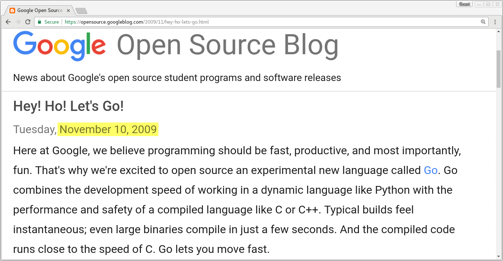
\includegraphics[width=0.9\linewidth]{announcement}
  \end{center}

  \vspace{-0.4\baselineskip}
  \fullvfill
  \hfill
  \begin{minipage}{\linewidth}
    \raggedright
    \tiny
    Image adapted from:
    \fullcite{GoAnnounce}
  \end{minipage}

  \note{
    From Donovan15:

    \begin{itemize}
    \item ``announced in November 2009''
    \end{itemize}
  }
\end{frame}

\subsection{Ancestors}

\begin{frame}[t]
  \frametitle{Ancestors}

  Go builds on other languages:
  \begin{itemize}
  \item borrows good ideas
  \item avoids features that lead to complexity/unreliability
  \end{itemize}

  \vspace{\baselineskip}
  Let's look at some examples\dots

  \note{
    From Donovan15:

    \begin{itemize}
    \item borrows good ideas
    \item avoids features that lead to overly complex and unreliable code
    \end{itemize}
  }
\end{frame}

\begin{frame}[t,fragile]
  \frametitle{Ancestor: C}

  \begin{tabular}{ll}
    \cellcolor{macewan}
    \rotatebox{90}{\bfseries\color{white}\hspace{-1mm}C} & \cellcolor{macewan!10}
\begin{lstlisting}[basicstyle={\scriptsize\ttfamily},language=c]
// basic data types
float fahrenheit, celsius;

// expression syntax
fahrenheit = 22;
celsius = (fahrenheit - 32) * 5.0 / 9.0;

// control-flow statements
if (celsius < 0) {
    printf("it's freezing!\n");
}
\end{lstlisting} \\
                                                         & \\
    \cellcolor{macewan}
    \rotatebox{90}{\bfseries\color{white}\hspace{-1mm}Go} & \cellcolor{macewan!10}
\begin{lstlisting}[basicstyle={\scriptsize\ttfamily},language=Golang]
var fahrenheit, celsius float32

fahrenheit = 22
celsius = (fahrenheit - 32) * 5.0 / 9.0

if celsius < 0 {
    fmt.Printf("it's freezing!\n")
}
\end{lstlisting} \\
  \end{tabular}

  \note{
    From Donovan15:

    \begin{itemize}
    \item shown: basic data types, expression syntax, control-flow statements
    \item not shown: call-by-value, pointers, compilation to efficient machine code
    \end{itemize}
  }
\end{frame}

\begin{frame}[t,fragile]
  \frametitle{Ancestor: \textit{Wirth} languages (1 of 2)}

  \begin{tabular}{ll}
    \cellcolor{macewan}
    \rotatebox{90}{\bfseries\color{white}\hspace{-7mm}Pascal} & \cellcolor{macewan!10}
\begin{lstlisting}[basicstyle={\scriptsize\ttfamily},language={Pascal}]
unit amazinglibrary;
(* interface & implementation both exist in one file *)

interface
    (* exported variables and functions *)

implementation
    (* definitions *)
\end{lstlisting} \\
                                                              & \\
    \cellcolor{macewan}
    \rotatebox{90}{\bfseries\color{white}\hspace{-2mm}Go} & \cellcolor{macewan!10}
\begin{lstlisting}[basicstyle={\scriptsize\ttfamily},language=Golang]
package amazinglibrary

// interface & implementation both exist in one file
\end{lstlisting}
  \end{tabular}

  \note{
    From Donovan15:

    \begin{itemize}
    \item package concept, interface \& implementation in one file
    \end{itemize}
  }
\end{frame}

\begin{frame}[t,fragile]
  \frametitle{Ancestor: \textit{Wirth} languages (2 of 2)}

  \begin{tabular}{ll}
    \cellcolor{macewan}
    \rotatebox{90}{\bfseries\color{white}\hspace{-7mm}Pascal} & \cellcolor{macewan!10}
\begin{lstlisting}[basicstyle={\scriptsize\ttfamily},language={Pascal}]
program someprogram;

(* programs can include a unit using "uses"... *)
uses
    (* units used... *)
    amazinglibrary;
\end{lstlisting} \\
                                                              & \\
    \cellcolor{macewan}
    \rotatebox{90}{\bfseries\color{white}\hspace{-2mm}Go} & \cellcolor{macewan!10}
\begin{lstlisting}[basicstyle={\scriptsize\ttfamily},language=Golang]
package main

// packages can include packages using "import"...
import (
    // packages used...
    "amazinglibrary"
)
\end{lstlisting}
  \end{tabular}

  \note{
    From Donovan15:

    \begin{itemize}
    \item syntax for packages, imports, declarations
    \end{itemize}
  }
\end{frame}

\begin{frame}[t,fragile]
  \frametitle{Ancestor: Oberon-2}

  \begin{tabular}{ll}
    \cellcolor{macewan}
    \rotatebox{90}{\bfseries\color{white}\hspace{-10mm}Oberon-2} & \cellcolor{macewan!10}
\begin{lstlisting}[basicstyle={\scriptsize\ttfamily},language={Oberon-2}]
(* syntax for method declaration *)
PROCEDURE (t: Tree) Lookup* (name: ARRAY OF CHAR): Tree;
    VAR p: Tree;
BEGIN p := t;
    WHILE (p # NIL) & (name # p.name^) DO
        IF name < p.name^ THEN p := p.left ELSE p := p.right END
    END;
    RETURN p
END Lookup;
\end{lstlisting} \\
                                                                 & \\
    \cellcolor{macewan}
    \rotatebox{90}{\bfseries\color{white}\hspace{-1mm}Go} & \cellcolor{macewan!10}
\begin{lstlisting}[basicstyle={\scriptsize\ttfamily},language=Golang]
func (t *Node) Lookup(name string) Tree {
    var p Tree
    p = t
    for p != nil && name != p.name {
        if name < p.name { p = p.left } else { p = p.right }
    }
    return p
}
\end{lstlisting}
  \end{tabular}

  \fullvfill
  \hfill
  \begin{minipage}{\linewidth}
    \raggedright
    \footnotesize
    Source:
    \fullcite{GoEvolution}
  \end{minipage}

  \note{
    From Donovan15:

    \begin{itemize}
    \item syntax for method declarations
      \begin{itemize}
      \item originally from \textit{Object} Oberon
      \end{itemize}
    \end{itemize}
  }
\end{frame}

\begin{frame}[t]
  \frametitle{Ancestors: Summary}

  \includegraphics[width=\linewidth]{ancestors}

  \fullvfill
  \hfill
  \begin{minipage}{\linewidth}
    \raggedright
    \footnotesize
    Adapted from:
    \fullcite{Donovan15}
  \end{minipage}

  \note{
    From Donovan15:

    \begin{itemize}
    \item CSP (Communicating Sequential Processes): a formal language for describing fundamental concepts of concurrency
      \begin{itemize}
      \item communication and synchronization using channels
      \end{itemize}
    \end{itemize}
  }
\end{frame}

\section{What is Go?}
\subsection*{}

\begin{frame}[t]
  \frametitle{Outline}

  \tableofcontents[currentsection]
\end{frame}

\begin{frame}[t]
  \frametitle{Go is a \underbar{project}}

  Components:

  \begin{enumerate}
  \item language
  \item standard libraries
  \item tools
  \end{enumerate}

  \vspace{\baselineskip}

  Moreover\dots\dots
  \begin{itemize}
  \item open source
  \item portable
  \item general-purpose
  \end{itemize}

  \note{
    \begin{itemize}
    \item open source \underbar{project}
      \begin{itemize}
      \item compiler \& libraries \& tools (code): BSD license
        \begin{quote}
          BSD licenses are a family of permissive free software licenses, imposing minimal restrictions on the redistribution of covered software.
          This is in contrast to copyleft licenses, which have reciprocity share-alike requirements.
          The original BSD license was used for its namesake, the Berkeley Software Distribution (BSD), a Unix-like operating system.
          \begin{flushright}
            Source: Wikipedia [BSD licenses]
          \end{flushright}
        \end{quote}
      \item much of the non-code: Creative Commons Attribution 3.0 License
      \end{itemize}
    \item portable
      \begin{itemize}
      \item for 1.8: binaries for\dots
        \begin{itemize}
        \item macOS
        \item Linux: 386, amd64, armv6l, ppc64le, s390x
        \item Windows: 386, amd64
        \item FreeBSD: 386, amd64
        \end{itemize}
      \item applications, too: cross-compile for these architectures
      \end{itemize}
    \item general purpose
      \begin{itemize}
      \item well-suited for building infrastructure, e.g., networked servers, web services
      \item well-suited for ``tools'' for programmers
      \item various domains: graphics, mobile applications, machine learning
      \end{itemize}
    \end{itemize}
  }
\end{frame}

\subsection{Language}

\begin{frame}[t]
  \frametitle{Go: Language}

  Goals:

  \begin{itemize}
  \item expressive
  \item effective for writing reliable \& robust programs
  \item efficient compilation
  \item efficient execution
  \end{itemize}
\end{frame}

\begin{frame}[t]
  \frametitle{Go: Language: Features}

  Some features:

  \begin{itemize}
  \item packages
  \item strong type system
  \item garbage collection
  \item system call interface
  \item concurrency
  \item object-orientation programming
  \end{itemize}

  \note{
    From Donovan15:

    \begin{itemize}
    \item strong type system
      \begin{itemize}
      \item not terribly complex
      \item balanced expressiveness with safety
      \item first-class functions: can be arguments, return values, \dots; treated as other values
      \item lexical scope: static scoping: think blocks\dots (like C)
      \item immutable strings (often encoded as UTF-8)
      \end{itemize}
    \item garbage collection: automatic memory management
    \item system call interface
      \begin{itemize}
      \item portability?
      \end{itemize}
    \item concurrency: new/efficient facilities (based on CSP)
      \begin{itemize}
      \item variable-sized stacks in lightweight threads
      \end{itemize}
    \item OOP:
      \begin{itemize}
      \item selected features from OOP
      \item unusually flexible
      \end{itemize}
    \end{itemize}
  }
\end{frame}

\begin{frame}[t]
  \frametitle{Go: Language: Omitted features}

  Omissions:

  \begin{itemize}
  \item implicit numeric conversions
  \item constructors/destructors
  \item operator overloading
  \item default parameter values
  \item inheritance
  \item generics
  \item exceptions
  \item macros
  \item function annotations
  \end{itemize}
\end{frame}

\subsection{Tools}

\begin{frame}[t]
  \frametitle{Go: Tools: Introduction}

  On the topic of Go's legacy:
  \begin{quote}
    I think it's the tooling that has grown, not in spite of the language, but as a deliberate symbiosis, which deserves recognition.
    \dots{}
    I think that \texttt{gofmt} deserves most of the credit here.

    \begin{flushright}
      \begin{minipage}{0.75\linewidth}
        \raggedright
        \footnotesize
        Source:
        \fullcite{GoLegacy}
      \end{minipage}
    \end{flushright}
  \end{quote}

  \note{
    In his talk, he also suggested that Go might be remembered for
    \begin{itemize}
    \item interfaces
    \item Goroutines
    \end{itemize}

    Tooling was just one of the three ideas.
  }
\end{frame}

\begin{frame}[t]
  \frametitle{Go: Tools: \texttt{go tool}}

  Go has a variety of integrated tools.

  \vspace{\baselineskip}
  Tools available through \texttt{go tool} in Go 1.8:

  \begin{center}
    \begin{columns}[T]
      \begin{column}{0.15\linewidth}
        \texttt{addr2line} \\
        \texttt{api} \\
        \texttt{asm} \\
        \texttt{cgo} \\
        \texttt{compile} \\
        \texttt{cover}
      \end{column}
      \begin{column}{0.15\linewidth}
        \texttt{dist} \\
        \texttt{doc} \\
        \texttt{fix} \\
        \texttt{gofmt} \\
        \texttt{link} \\
        \texttt{nm}
      \end{column}
      \begin{column}{0.15\linewidth}
        \texttt{objdump} \\
        \texttt{pack} \\
        \texttt{pprof} \\
        \texttt{tour} \\
        \texttt{trace} \\
        \texttt{vet}
      \end{column}
    \end{columns}
  \end{center}

  \note{
    \tiny
    From https://golang.org/cmd/:
    \begin{tabular}{lp{3.5in}}
      addr2line &   minimal simulation of the GNU addr2line tool (just enough to support pprof) \\
      api &	    computes exported API of a set of Go packages \\
      asm &	    typically invoked as ``go tool asm,'' assembles the source file into an object file named for the basename of the argument source file with a .o suffix \\
      cgo &	    enables the creation of Go packages that call C code \\
      compile &	    typically invoked as ``go tool compile,'' compiles a single Go package comprising the files named on the command line \\
      cover &	    analyzing the coverage profiles generated by 'go test -coverprofile=cover.out' \\
      dist &	    bootstrapping tool for the Go distribution \\
      doc &	    typically invoked as ``go doc,'' shows documentation for a package, symbol, and/or method \\
      fix &	    finds Go programs that use old APIs and rewrites them to use newer ones \\
      go &	    tool for managing Go source code \\
      gofmt &	    formats Go programs \\
      link &	    typically invoked as ``go tool link,'' reads the Go archive or object for a package main, along with its dependencies, and combines them into an executable binary \\
      nm &	    lists the symbols defined or used by an object file, archive, or executable \\
      objdump &	    disassembles executable files \\
      pack &	    simple version of the traditional Unix ar tool \\
      pprof &	    interprets and displays profiles of Go programs \\
      trace &	    viewing trace files \\
      vet &	    examines Go source code and reports suspicious constructs, such as Printf calls whose arguments do not align with the format string \\
    \end{tabular}
  }
\end{frame}

\begin{frame}[t]
  \frametitle{Go: Tools: External}

  Many other tools exist, too, e.g.,

  \begin{itemize}
  \item \texttt{callgraph}
  \item \texttt{goimports}
  \item \texttt{gorename}
  \item \texttt{guru}
  \item \texttt{present}
  \end{itemize}

  \note{
    \begin{itemize}
    \item \texttt{callgraph}: for reporting the call graph
    \item \texttt{goimports}: for updating your import lines
    \item \texttt{gorename}: for renaming identifiers in a type-safe way
    \item \texttt{guru}: for answering questions about source code
    \item \texttt{present}: for displaying slide presentations and articles
  \end{itemize}
  }
\end{frame}

\subsection{Standard libraries}

\begin{frame}[t]
  \frametitle{Go: Standard libraries}

  Go has an extensive standard library ($\sim$140 packages).

  \vspace{\baselineskip}
  Examples:

  \vspace{\baselineskip}
  \begin{tabular}{ll}
    \bfseries{}Package  & \bfseries{}Description \\
    \texttt{archive/zip} & reading/writing ZIP files \\
    \texttt{compress/bzip2} & bzip2 decompression \\
    \texttt{crypto/elliptic} & several elliptic curves over prime fields \\
    \texttt{image/png} & PNG image decoder/encoder \\
    \texttt{net/smtp} & Simple Mail Transfer Protocol \\
    \texttt{syscall} & interface to low-level OS primitives \\
  \end{tabular}

  \note{
    \begin{itemize}
    \item ``often described as `batteries included''
      \begin{itemize}
      \item clean building blocks/APIS for I/O, text processing, graphics, cryptography, networking, and distributed applications
      \item support for standard file formats and protocols
      \end{itemize}
    \end{itemize}
  }
\end{frame}

\begin{frame}[t]
  \frametitle{Go: Standard libraries: Lines}

  \includegraphics[width=\linewidth]{gocode}

  \note{
    \begin{itemize}
    \item looked at git releases from 1 (2012) to 1.8 (2017) -- 5 years
    \item lines within .go files
      \begin{itemize}
      \item no attempt to isolate just lines of code
      \end{itemize}
    \item within \texttt{src/pkg} (1 to 1.3) and \texttt{src} (1.4+)
    \item attempted to filter out\dots
      \begin{itemize}
      \item vendor
      \item runtime
      \item cmd
      \item test
      \item anything platform/architecture specific
      \end{itemize}
    \end{itemize}
  }
\end{frame}

\section{Workshop}
\subsection{Schedule}

\begin{frame}[t]
  \frametitle{Outline}

  \tableofcontents[currentsection]
\end{frame}

\begin{frame}[t]
  \frametitle{Schedule: Morning}

  Schedule for the morning:

  \begin{description}
  \item[9:00] Welcome and opening remarks
  \item[9:30] Basics of Go
  \item[9:55] Types
  \item[10:20] Functions \& standard library basics
  \item[10:45] Control structures
  \item[11:10] Pointers
  \item[11:25] Exercises and questions
  \end{description}
\end{frame}

\begin{frame}[t]
  \frametitle{Schedule: Afternoon}

  Schedule for the afternoon:

  \begin{description}
  \item[1:00] Maps
  \item[1:25] Slices
  \item[1:50] User-defined types \& structs
  \item[2:15] Methods
  \item[2:40] Interfaces
  \item[3:05] Error
  \item[4:00] Comprehensive exercises
  \item[5:00] Closing remarks
  \end{description}
\end{frame}

\subsection{Presenters and mentors}

\begin{frame}[t]
  \frametitle{Presenters and mentors}

  List of presenters/mentors:

  \begin{itemize}
  \item Brett McKay
  \item Gerrit Renker
  \item James Bell
  \item Jordan Torbiak
  \item Matthias Stone
  \item Nathan Youngman
  \item Łukasz Różycki
  \end{itemize}
\end{frame}

\end{document}